% !TEX root = ../proyect.tex

\chapter{Dise\~no e Implementaci\'on}\label{cap08}

\section{Arquitectura del Sistema}\label{sec:arquitectura}

\subsection{Visi\'on general}\label{subsec:vision-general}

BargAIN sigue una arquitectura de \textbf{tres capas} cl\'asica (presentaci\'on, l\'ogica de
negocio y datos), desplegada mediante contenedores Docker y organizada internamente seg\'un los
principios de la \textbf{arquitectura hexagonal} (puertos y adaptadores). Esta elecci\'on permite
desacoplar la l\'ogica de dominio de los detalles de infraestructura --- bases de datos, APIs
externas, brokers de mensajer\'ia --- facilitando el testing independiente de cada componente.

La arquitectura global se divide en cinco bloques principales:

\begin{enumerate}
  \item \textbf{Aplicaci\'on cliente:} React Native (Expo) para iOS y Android, con una aplicaci\'on
    web React para el Portal Business de PYMEs.
  \item \textbf{API Backend:} Django REST Framework como n\'ucleo de la l\'ogica de negocio,
    expuesto bajo HTTPS mediante Gunicorn + Nginx.
  \item \textbf{Capa de datos:} PostgreSQL 16 con extensi\'on PostGIS 3.4 para consultas
    geoespaciales.
  \item \textbf{Capa de tareas as\'incronas:} Celery con Redis como broker, para scraping
    peri\'odico, env\'io de notificaciones, procesamiento OCR y c\'alculos del optimizador.
  \item \textbf{Integraciones y servicios auxiliares:} Google Gemini API (asistente LLM),
    OpenRouteService (c\'alculo de distancias reales), Google Cloud Vision API (OCR) y Sentry
    (monitorizaci\'on de errores).
\end{enumerate}

\subsection{Patr\'on de organizaci\'on interna del backend}\label{subsec:patron-backend}

Cada aplicaci\'on Django del backend sigue una estructura modular consistente:

\begin{verbatim}
apps/<modulo>/
|-- models.py          # Entidades de dominio (ORM)
|-- serializers.py     # Transformacion de datos (entrada/salida)
|-- views.py           # ViewSets y vistas (controladores)
|-- urls.py            # Rutas del modulo
|-- services.py        # Logica de negocio
|-- tasks.py           # Tareas Celery asincronas
|-- permissions.py     # Logica de autorizacion
`-- tests/
\end{verbatim}

La separaci\'on entre \texttt{views.py} y \texttt{services.py} es deliberada: los ViewSets se
limitan a la gesti\'on HTTP (autenticaci\'on, serializaci\'on, c\'odigos de respuesta), mientras
que la l\'ogica de negocio reside exclusivamente en los servicios, lo que permite invocarla desde
tareas Celery o tests sin simular peticiones HTTP.

La Figura~\ref{fig:arquitectura-capas} resume la distribuci\'on por capas de la soluci\'on.

\begin{figure}[htbp]
\centering
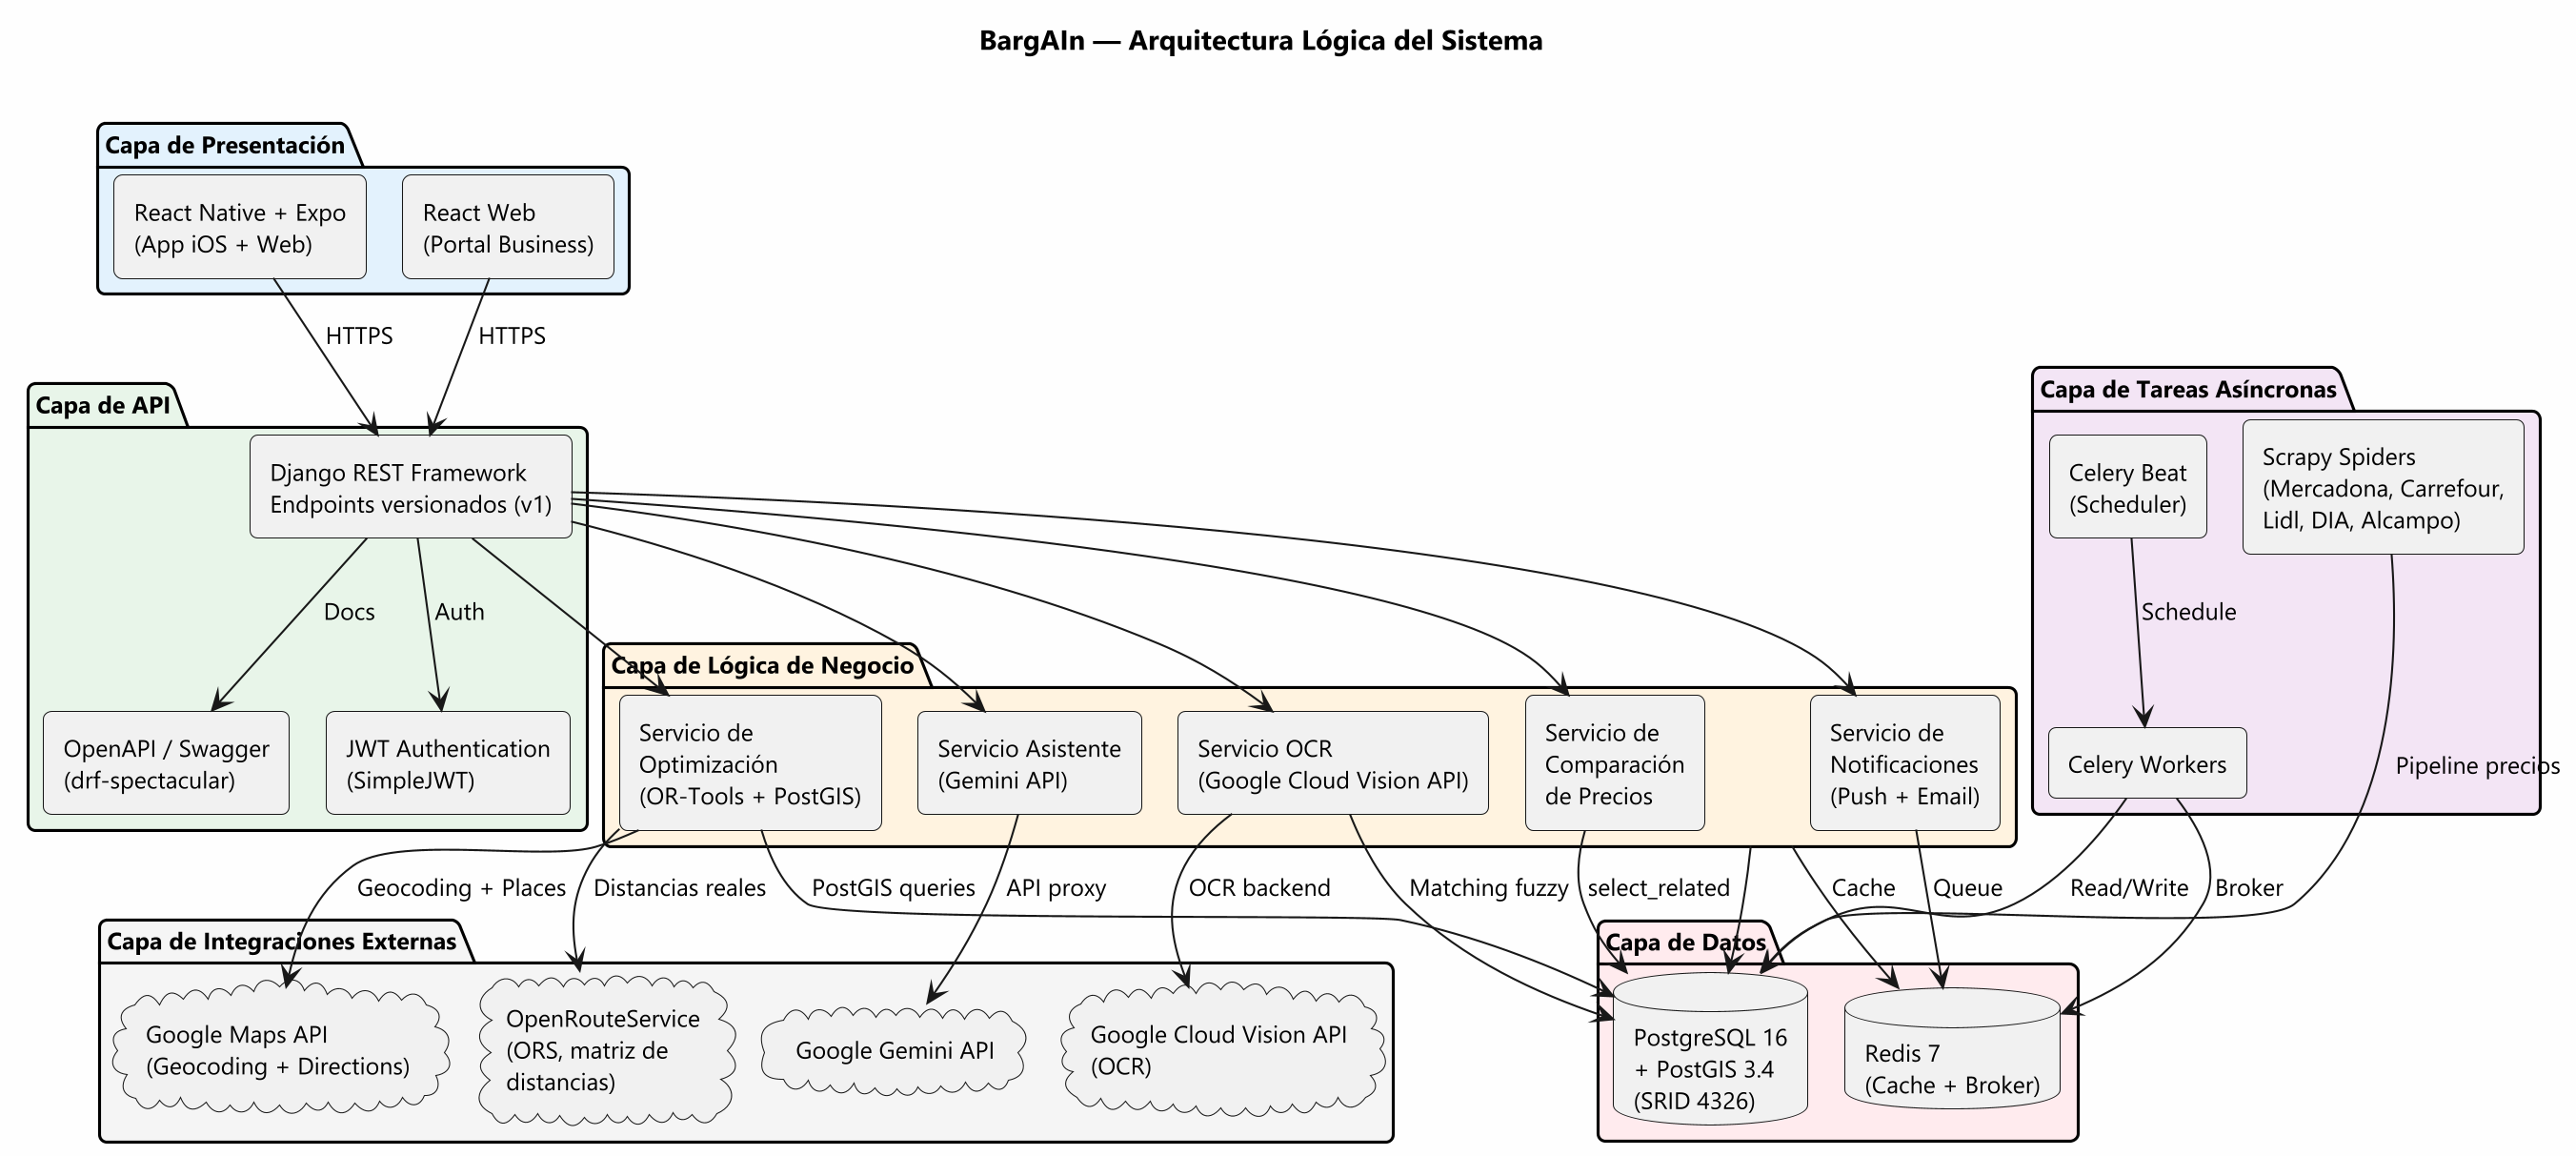
\includegraphics[width=0.92\textwidth]{../diagramas/arquitectura/arquitectura-capas.png}
\caption{Arquitectura por capas de BargAIN}
\label{fig:arquitectura-capas}
\end{figure}

\subsection{Comunicaci\'on entre componentes}\label{subsec:comunicacion}

\begin{itemize}
  \item \textbf{Frontend \textrightarrow{} Backend:} API REST con autenticaci\'on JWT. Axios
    gestiona la renovaci\'on autom\'atica del token de acceso ante un \texttt{401 Unauthorized}.
  \item \textbf{Backend \textrightarrow{} Celery:} Encolar tareas mediante \texttt{.delay()} o
    \texttt{.apply\_async()} sobre el broker Redis.
  \item \textbf{Backend \textrightarrow{} PostgreSQL:} Django ORM con consultas geoespaciales
    mediante \texttt{django.contrib.gis}.
  \item \textbf{Backend \textrightarrow{} APIs externas:} Clientes HTTP aislados en
    \texttt{apps/<modulo>/clients/} para Google Maps, Gemini API y ORS.
\end{itemize}

\section{Modelo de Datos}\label{sec:modelo-datos}

\subsection{M\'odulo de usuarios}\label{subsec:modelo-usuarios}

El modelo \texttt{User} extiende \texttt{AbstractBaseUser} de Django para permitir el login
mediante email. Se definen tres roles: \texttt{consumer}, \texttt{business} y \texttt{admin}.
El campo \texttt{default\_location} utiliza \texttt{PointField(SRID=4326)}.

Las preferencias de optimizaci\'on (\texttt{w\_precio}, \texttt{w\_distancia}, \texttt{w\_tiempo})
se almacenan como decimales con restricci\'on de que su suma sea igual a 1.0, validada a nivel de
serializer:

\begin{verbatim}
def validate(self, data: dict) -> dict:
    weights = [
        data.get('weight_price', 0),
        data.get('weight_distance', 0),
        data.get('weight_time', 0),
    ]
    if abs(sum(weights) - 1.0) > 0.001:
        raise serializers.ValidationError(
            "Los pesos de optimizacion deben sumar exactamente 1.0"
        )
    return data
\end{verbatim}

\subsection{M\'odulo de productos}\label{subsec:modelo-productos}

La b\'usqueda de productos por nombre utiliza \textbf{matching fuzzy} mediante la extensi\'on
PostgreSQL \texttt{pg\_trgm} (trigramas). El campo \texttt{normalized\_name} almacena el nombre
normalizado (min\'usculas, sin tildes, sin caracteres especiales) con \'indices GIN de trigramas:

\begin{verbatim}
def search_products(query: str, limit: int = 20) -> QuerySet[Product]:
    return (
        Product.objects
        .annotate(similarity=TrigramSimilarity(
            'normalized_name', normalize(query)))
        .filter(similarity__gt=0.3, is_active=True)
        .order_by('-similarity')[:limit]
    )
\end{verbatim}

\subsection{M\'odulo de tiendas}\label{subsec:modelo-tiendas}

El campo \texttt{location} de \texttt{Store} es un \texttt{PointField} con \'indice GiST para
b\'usquedas geoespaciales eficientes:

\begin{verbatim}
def get_stores_in_radius(
    lat: float, lng: float, radius_km: float
) -> QuerySet[Store]:
    user_location = Point(lng, lat, srid=4326)
    return (
        Store.objects
        .filter(
            location__dwithin=(user_location, D(km=radius_km)),
            is_active=True
        )
        .annotate(distance=Distance('location', user_location))
        .order_by('distance')
    )
\end{verbatim}

El uso de \texttt{ST\_DWithin} en lugar de \texttt{ST\_Distance} en el \texttt{WHERE} es
deliberado: \texttt{ST\_DWithin} puede aprovechar el \'indice GiST, mientras que calcular
distancias en el filtro forzar\'ia un escaneo completo de la tabla.

\subsection{M\'odulo de precios}\label{subsec:modelo-precios}

El hist\'orico de precios se materializa autom\'aticamente: cada precio es inmutable una vez
creado. La actualizaci\'on de un precio supone la inserci\'on de un nuevo registro. Una tarea
Celery peri\'odica (\texttt{expire\_stale\_prices}) marca como expirados los precios de scraping
con m\'as de 48 horas de antig\"uedad y los de crowdsourcing con m\'as de 24 horas.

\subsection{M\'odulo del optimizador}\label{subsec:modelo-optimizador}

El m\'odulo del optimizador incluye tres entidades relacionales para almacenar el resultado de la
optimizaci\'on de forma trazable:

\begin{itemize}
  \item \textbf{\texttt{OptimizationResult}:} resultado global con pesos, modo y m\'etricas
    totales. Incluye \texttt{route\_data} JSONB para compatibilidad de lectura r\'apida.
  \item \textbf{\texttt{OptimizationRouteStop}:} cada parada de la ruta con tienda, orden,
    distancia, tiempo y subtotal.
  \item \textbf{\texttt{OptimizationRouteStopItem}:} \'item concreto por parada, con producto
    resuelto, precio elegido, texto original y puntuaci\'on de similitud.
\end{itemize}

\subsection{\'Indices clave}\label{subsec:indices}

\begin{table}[h]
\caption{\'Indices principales de la base de datos}
\label{tab:indices}
\centering
\begin{tabular}{|l|l|l|p{5cm}|}
\hline
\textbf{Tabla} & \textbf{Columna(s)} & \textbf{Tipo} & \textbf{Justificaci\'on} \\
\hline
\texttt{store} & \texttt{location} & GiST &
  B\'usquedas geoespaciales por radio \\
\texttt{price} & \texttt{(product, store, created\_at)} & B-Tree &
  Hist\'orico y precio actual \\
\texttt{price} & \texttt{expires\_at} & B-Tree parcial &
  Filtrar precios vigentes \\
\texttt{product} & \texttt{normalized\_name} & GIN (trigram) &
  B\'usqueda fuzzy por nombre \\
\texttt{shopping\_list\_item} & \texttt{(shopping\_list, is\_checked)} & B-Tree &
  \'Items pendientes \\
\hline
\end{tabular}
\end{table}

\subsection{Modelo entidad-relaci\'on}\label{subsec:modelo-er}

La Figura~\ref{fig:modelo-er} muestra el diagrama entidad-relaci\'on completo de la base de datos.

\begin{figure}[htbp]
\centering

\includegraphics[width=\textwidth]{../diagramas/er/modelo-er.png}
\caption{Diagrama entidad-relaci\'on de BargAIN}
\label{fig:modelo-er}
\end{figure}

\subsection{Diagrama de clases}\label{subsec:modelo-clases}

La Figura~\ref{fig:modelo-clases} detalla las clases principales del dominio y sus relaciones.

\begin{figure}[htbp]
\centering

\includegraphics[width=\textwidth]{../diagramas/clases/modelo-clases.png}
\caption{Diagrama de clases del dominio}
\label{fig:modelo-clases}
\end{figure}

\section{Dise\~no de la API REST}\label{sec:api}

\subsection{Estructura general}\label{subsec:api-estructura}

La API sigue las convenciones REST y est\'a versionada bajo el prefijo \texttt{/api/v1/}. Todos
los endpoints requieren autenticaci\'on JWT salvo los de registro y login. Las respuestas siguen
el formato unificado:

\begin{verbatim}
// Respuesta exitosa
{
  "success": true,
  "data": { ... },
  "meta": { "count": 42, "page": 1, "page_size": 20 }
}

// Respuesta de error
{
  "success": false,
  "error": {
    "code": "STORE_NOT_FOUND",
    "message": "No se encontraron tiendas en el radio especificado",
    "details": {}
  }
}
\end{verbatim}

\subsection{Endpoints principales}\label{subsec:api-endpoints}

\begin{table}[h]
\caption{Endpoints de autenticaci\'on y usuarios}
\label{tab:api-auth}
\centering
\begin{tabular}{|l|p{6cm}|p{5cm}|}
\hline
\textbf{M\'etodo} & \textbf{Endpoint} & \textbf{Descripci\'on} \\
\hline
\texttt{POST} & \texttt{/api/v1/auth/register/} & Registro de nuevo usuario \\
\texttt{POST} & \texttt{/api/v1/auth/login/} & Login: access + refresh token \\
\texttt{POST} & \texttt{/api/v1/auth/token/refresh/} & Renovar access token \\
\texttt{POST} & \texttt{/api/v1/auth/logout/} & Invalidar refresh token \\
\texttt{GET/PATCH} & \texttt{/api/v1/users/me/} & Perfil del usuario autenticado \\
\texttt{GET/PATCH} & \texttt{/api/v1/users/me/preferences/} & Preferencias de optimizaci\'on \\
\hline
\end{tabular}
\end{table}

\begin{table}[h]
\caption{Endpoints del optimizador, OCR y asistente}
\label{tab:api-core}
\centering
\begin{tabular}{|l|p{6cm}|p{5cm}|}
\hline
\textbf{M\'etodo} & \textbf{Endpoint} & \textbf{Descripci\'on} \\
\hline
\texttt{POST} & \texttt{/api/v1/optimize/} & Calcular o recalcular ruta \'optima \\
\texttt{GET} & \texttt{/api/v1/optimize/?shopping\_list\_id=\{id\}} &
  Cargar \'ultima ruta persistida \\
\texttt{POST} & \texttt{/api/v1/ocr/scan/} &
  Procesar imagen y devolver \'items reconocidos \\
\texttt{GET/POST} & \texttt{/api/v1/assistant/conversations/} &
  Listar y crear conversaciones \\
\texttt{POST} & \texttt{/api/v1/assistant/conversations/\{id\}/messages/} &
  Enviar mensaje al asistente \\
\hline
\end{tabular}
\end{table}

\subsection{Autenticaci\'on y autorizaci\'on}\label{subsec:api-auth}

Se implementa un sistema de permisos a tres niveles:

\begin{itemize}
  \item \textbf{\texttt{IsAuthenticated}:} Aplicado por defecto a todos los endpoints privados.
  \item \textbf{\texttt{IsBusinessOwner}:} Permite operar solo sobre el perfil de negocio propio.
  \item \textbf{\texttt{IsAdminUser}:} Para endpoints de administraci\'on del sistema.
  \item \textbf{\texttt{IsShoppingListOwnerOrShared}:} Permite acceso al propietario y
    colaboradores invitados.
\end{itemize}

Los tokens JWT se generan con \texttt{djangorestframework-simplejwt}. El token de acceso tiene
validez de 60 minutos y el de refresco de 7 d\'ias con rotaci\'on autom\'atica.

\section{Implementaci\'on del Backend}\label{sec:implementacion-backend}

\subsection{M\'odulo de notificaciones}\label{subsec:impl-notificaciones}

El m\'odulo gestiona el buz\'on de notificaciones del usuario (inbox) y el env\'io de
notificaciones push mediante \textbf{Expo Push Notifications}. Las entregas se procesan
as\'incronamente con tareas Celery.

\begin{itemize}
  \item \textbf{\texttt{Notification}:} Registro persistente con \texttt{notification\_type}
    (\texttt{price\_alert}, \texttt{new\_promo}, \texttt{shared\_list\_changed},
    \texttt{business\_approved}, \texttt{business\_rejected}), campos \texttt{title}/\texttt{body},
    bandera \texttt{is\_read}, \texttt{data} JSONB para payload variable, \texttt{action\_url}
    para deep links y \texttt{deleted\_at} para soft-delete.
  \item \textbf{\texttt{UserPushToken}:} Token Expo registrado por dispositivo. La clave \'unica
    \texttt{(user, device\_id)} evita duplicados al reinstalar la app.
\end{itemize}

\subsection{M\'odulo de portal business}\label{subsec:impl-business}

\begin{itemize}
  \item \textbf{\texttt{BusinessProfile}:} Perfil verificable con \texttt{tax\_id} (CIF/NIF
    \'unico), estado de verificaci\'on y umbral de alerta de competidor
    (\texttt{price\_alert\_threshold\_pct}).
  \item \textbf{\texttt{Promotion}:} Promoci\'on temporal de un producto en una tienda. Restricci\'on
    parcial \'unica \texttt{(product, store) WHERE is\_active} garantiza que no existan dos
    promociones activas para el mismo par.
\end{itemize}

La tarea Celery \texttt{check\_competitor\_prices} se ejecuta cada 6 horas y alerta al propietario
cuando detecta diferencias superiores al umbral configurado.

\section{El Algoritmo de Optimizaci\'on de Rutas}\label{sec:algoritmo}

\subsection{Formulaci\'on del problema}\label{subsec:formulacion}

El algoritmo de optimizaci\'on es la aportaci\'on t\'ecnica central del TFG. El problema es una
variante del \textbf{Vehicle Routing Problem (VRP)} con objetivos m\'ultiples, resuelto mediante
una soluci\'on heur\'istica eficiente.

\textbf{Entrada:}
\begin{itemize}
  \item Lista de la compra $L = \{i_1, i_2, \ldots, i_n\}$ (n \'items textuales)
  \item Ubicaci\'on del usuario $u = (lat, lng)$
  \item Radio m\'aximo $r$ (km), n\'umero m\'aximo de paradas $k$ (1--4)
  \item Pesos de preferencia $w_{precio}$, $w_{distancia}$, $w_{tiempo}$ (suman 1.0)
\end{itemize}

\textbf{Salida:} Top-3 asignaciones de \'items resueltos a tiendas que minimizan la funci\'on
de coste.

\subsection{Funci\'on de scoring multicriterio}\label{subsec:scoring}

\begin{equation}
  \text{Score}(A) = w_{precio} \cdot \text{ahorro\_norm}(A)
                 - w_{distancia} \cdot \text{dist\_extra\_norm}(A)
                 - w_{tiempo} \cdot \text{tiempo\_extra\_norm}(A)
\end{equation}

Donde \texttt{ahorro\_normalizado} = $(\text{coste\_single\_best} - \text{coste}(A)) /
\text{coste\_single\_best} \in [0, 1]$ y \texttt{distancia\_extra\_normalizada} = $\max(0,
\text{dist\_ruta}(A) - \text{dist\_single}) / (r \times 1{,}5)$.

\subsection{Pipeline de ejecuci\'on}\label{subsec:pipeline}

El algoritmo se ejecuta en seis fases secuenciales dentro de
\texttt{apps/optimizer/services.py}:

\begin{enumerate}
  \item \textbf{Fase 0 --- Resoluci\'on textual de \'items:} Preseleccion por trigramas sobre
    \texttt{Product.normalized\_name}, ranking fuzzy (\texttt{token\_set\_ratio}), y validaci\'on
    contextual por disponibilidad de precio.

  \item \textbf{Fase 1 --- Ingesta de precios candidatos:} Para cada producto resuelto, se
    obtienen los precios vigentes en tiendas dentro del radio con una sola consulta optimizada
    con \texttt{select\_related} y filtros geoespaciales.

  \item \textbf{Fase 2 --- Pre-filtrado de tiendas:} Se limita a 30 tiendas candidatas m\'aximo
    para controlar la explosi\'on combinatoria (C(30, 3) = 4.060 combinaciones para k=3).

  \item \textbf{Fase 3 --- Generaci\'on y evaluaci\'on de asignaciones:} Para cada combinaci\'on
    de tiendas, asignaci\'on greedy \'optima de \'items al menor precio disponible.

  \item \textbf{Fase 4 --- C\'alculo de distancias reales:} Matriz de distancias v\'ia
    \textbf{OpenRouteService (ORS)} en una sola petici\'on. Fallback haversine si ORS no est\'a
    disponible:

\begin{verbatim}
POST https://api.openrouteservice.org/v2/matrix/driving-car
Authorization: {ORS_API_KEY}

{
  "locations": [[lng1, lat1], [lng2, lat2], ...],
  "metrics": ["distance", "duration"],
  "units": "km"
}
\end{verbatim}

  \item \textbf{Fase 5 --- Scoring y ranking:} Normalizaci\'on de valores al rango [0, 1] y
    devoluci\'on de las top-3 asignaciones ordenadas por score descendente.
\end{enumerate}

\subsection{Diagrama de secuencia del optimizador}\label{subsec:secuencia-optimizador}

La Figura~\ref{fig:secuencia-optimizacion} ilustra el flujo de mensajes entre componentes
durante una petici\'on de optimizaci\'on.

\begin{figure}[htbp]
\centering

\includegraphics[width=0.95\textwidth]{../diagramas/secuencia/secuencia-optimizacion.png}
\caption{Diagrama de secuencia del proceso de optimizaci\'on de ruta}
\label{fig:secuencia-optimizacion}
\end{figure}

\subsection{Integraci\'on con OR-Tools}\label{subsec:ortools}

Para combinaciones complejas donde el problema de asignaci\'on supera la heur\'istica greedy, se
utiliza \textbf{OR-Tools de Google} para resolver el problema como programaci\'on lineal entera
(ILP), garantizando la optimalidad de la asignaci\'on de productos a tiendas dentro de un
subconjunto fijo de tiendas.

\subsection{Complejidad y rendimiento}\label{subsec:rendimiento}

\begin{table}[h]
\caption{Tiempos estimados de ejecuci\'on del optimizador}
\label{tab:rendimiento}
\centering
\begin{tabular}{|l|c|c|c|}
\hline
\textbf{Escenario} & \textbf{Tiendas} & \textbf{Combinaciones (k=3)} & \textbf{Tiempo} \\
\hline
Lista peque\~na (5 prod.) & $\leq 15$ & 455 & $<$ 1 s \\
Lista media (20 prod.) & $\leq 30$ & 4.060 & $<$ 3 s \\
Lista grande (50 prod.) & $\leq 30$ & 4.060 & $<$ 5 s \\
\hline
\end{tabular}
\end{table}

El umbral de 5 s (RNF-001) se cumple gracias a: pre-filtrado de tiendas, cach\'e de matriz de
distancias en Redis, y ejecuci\'on como tarea Celery as\'incrona.

\section{M\'odulo de Web Scraping}\label{sec:scraping}

El scraper es un \textbf{proyecto Scrapy independiente} (\texttt{scraping/}) desacoplado del
backend Django, que comunica con la base de datos a trav\'es de la API REST del propio backend.

Cada cadena requiere una estrategia diferente:

\begin{itemize}
  \item \textbf{Mercadona:} API interna (\texttt{uapi.mercadona.es}) no oficial pero estable,
    accesible mediante peticiones HTTP est\'andar.
  \item \textbf{Carrefour / Lidl / DIA:} Cat\'alogos con renderizado del lado del cliente (SPA),
    por lo que se usa \textbf{Playwright} para ejecutar el JavaScript y obtener el DOM hidratado.
\end{itemize}

Los spiders se programan con \textbf{Celery Beat}, con un delay m\'inimo de 2 segundos entre
peticiones consecutivas (regla de negocio RN-010).

\section{M\'odulo OCR}\label{sec:ocr}

El backend invoca \textbf{Google Cloud Vision API} con la imagen capturada por el usuario. La
decisi\'on de migrar desde Tesseract a Vision API se adopt\'o tras comprobar que Tesseract no
reconoce con suficiente claridad tickets y listas fotografiadas en condiciones reales:

\begin{verbatim}
from google.cloud import vision

def extract_text_from_image(image_bytes: bytes) -> list[str]:
    """Extrae lineas de texto mediante Google Cloud Vision API."""
    client = vision.ImageAnnotatorClient()
    image = vision.Image(content=image_bytes)
    response = client.text_detection(image=image)
    full_text = response.full_text_annotation.text
    return [line.strip() for line in full_text.splitlines() if line.strip()]
\end{verbatim}

Cada l\'inea extra\'ida se normaliza y se busca en el cat\'alogo mediante el servicio de matching
fuzzy de \texttt{apps/products}. Se devuelve una lista de candidatos con nivel de confianza.

\subsection{Diagrama de secuencia OCR}\label{subsec:secuencia-ocr}

La Figura~\ref{fig:secuencia-ocr} muestra el flujo de procesamiento desde la captura de imagen
hasta la inserci\'on de \'items en la lista.

\begin{figure}[htbp]
\centering
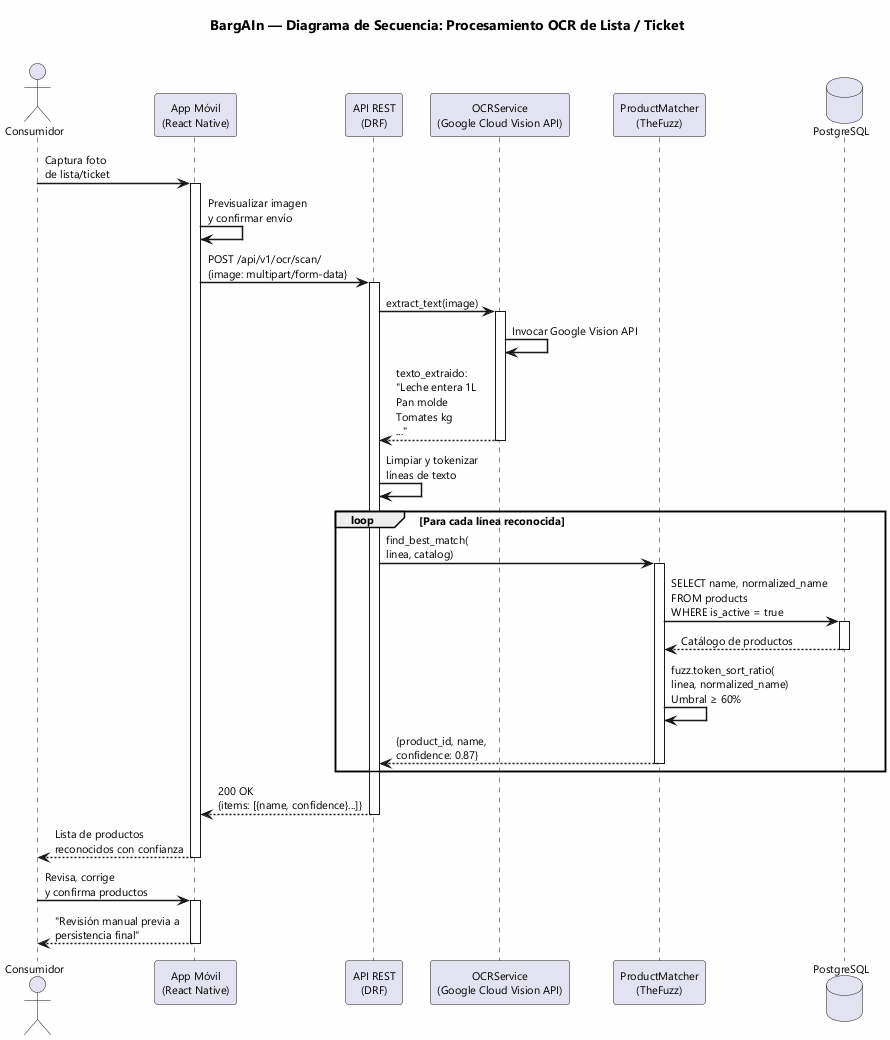
\includegraphics[width=0.95\textwidth]{../diagramas/secuencia/secuencia-ocr.png}
\caption{Diagrama de secuencia del flujo OCR}
\label{fig:secuencia-ocr}
\end{figure}

\section{Integraci\'on del Asistente LLM}\label{sec:asistente}

El asistente conversacional utiliza la \textbf{Google Gemini API}
(\texttt{gemini-2.0-flash-lite}) como modelo subyacente (ADR-008). El backend actúa como proxy,
añadiendo contexto de la compra del usuario al system prompt antes de enviar cada mensaje a la
API mediante el SDK \texttt{google-genai}.

Se aplica una \textbf{ventana deslizante} sobre el historial de mensajes (\'ultimos 20 mensajes
+ system prompt) para mantener el consumo de tokens controlado. El system prompt incluye un
guardrail que limita las respuestas a consultas de compra dom\'estica (RN-007).

\section{Infraestructura y Despliegue}\label{sec:infraestructura}

\subsection{Contenedores Docker}\label{subsec:docker}

Cada componente se ejecuta en un contenedor independiente, orquestados con Docker Compose:

\begin{itemize}
  \item \textbf{nginx:} Reverse proxy y servicio de est\'aticos.
  \item \textbf{backend:} Django + Gunicorn (3 workers).
  \item \textbf{celery-worker:} Workers para tareas as\'incronas.
  \item \textbf{celery-beat:} Scheduler de tareas peri\'odicas.
  \item \textbf{db:} PostgreSQL 16 + PostGIS.
  \item \textbf{redis:} Broker Celery + cach\'e.
\end{itemize}

Para el entorno de desarrollo se usa el modelo h\'ibrido (ADR-002): backend en Docker, frontend
nativo en el host. Docker volumes en Windows rompen el HMR de Metro/Expo, por lo que el frontend
no se dockeriza.

\subsection{Pipeline CI/CD}\label{subsec:cicd}

El repositorio incluye tres workflows de GitHub Actions:

\begin{itemize}
  \item \textbf{\texttt{ci-backend.yml}:} Ejecuta \texttt{ruff check}, \texttt{ruff format
    --check} y \texttt{pytest --cov} en cada push a cualquier rama.
  \item \textbf{\texttt{ci-frontend.yml}:} Ejecuta \texttt{eslint}, \texttt{prettier --check}
    y \texttt{jest --coverage} en cada push.
  \item \textbf{\texttt{ios-build.yml}:} Genera el \texttt{.ipa} unsigned mediante
    \texttt{expo prebuild} + \texttt{xcodebuild} en un runner \texttt{macos-latest}. El artefacto
    se descarga y se instala en el iPhone de demo con Sideloadly.
\end{itemize}

El deploy a staging se realiza mediante \textbf{Render Blueprints} (\texttt{render.yaml} en la
ra\'iz del repositorio), que define declarativamente 5 servicios. Cada push a \texttt{main}
dispara un redespliegue autom\'atico.

\subsection{Variables de entorno}\label{subsec:env}

La configuraci\'on sensible (claves API, credenciales de BD, secret key de Django) se gestiona
exclusivamente mediante variables de entorno, nunca hardcodeadas. Se proporciona
\texttt{.env.example} con los nombres de todas las variables requeridas.

\section{Dise\~no de la Interfaz de Usuario}\label{sec:ui}

\subsection{Sistema de dise\~no}\label{subsec:design-system}

El frontend define un sistema de dise\~no propio en \texttt{src/theme/} con los siguientes
tokens:

\begin{table}[h]
\caption{Paleta de colores del sistema de dise\~no}
\label{tab:colores}
\centering
\begin{tabular}{|l|l|l|}
\hline
\textbf{Token} & \textbf{Valor} & \textbf{Uso} \\
\hline
\texttt{primary} & \texttt{\#2E7D32} & Acciones principales, CTAs \\
\texttt{primaryLight} & \texttt{\#60AD5E} & Estados hover, fondos sutiles \\
\texttt{secondary} & \texttt{\#FF6F00} & Ahorros, destacados, ofertas \\
\texttt{surface} & \texttt{\#FAFAFA} & Fondo de tarjetas \\
\texttt{error} & \texttt{\#C62828} & Errores y alertas \\
\texttt{textPrimary} & \texttt{\#212121} & Texto principal \\
\texttt{textSecondary} & \texttt{\#757575} & Texto de apoyo \\
\hline
\end{tabular}
\end{table}

\textbf{Tipograf\'ia:} Inter (sans-serif) con escala modular. \textbf{Espaciado:} Escala de 4px.

\subsection{Pantallas principales}\label{subsec:pantallas}

La aplicaci\'on se estructura en cinco pesta\~nas principales:

\begin{enumerate}
  \item \textbf{Inicio / Dashboard:} Resumen de la lista activa, precio estimado en la tienda
    m\'as barata cercana, acceso r\'apido al asistente y alertas activas.
  \item \textbf{Mi Lista:} Gesti\'on de la lista activa con buscador de autocompletado, grupos
    por categor\'ia, swipe-to-delete/check y bot\'on de optimizar ruta.
  \item \textbf{Explorar:} Mapa interactivo con marcadores de tiendas y panel inferior
    deslizable con detalles de la tienda seleccionada.
  \item \textbf{Optimizador:} Sliders de pesos, cards comparativas de las top-3 rutas y
    visualizaci\'on de la ruta en mapa con polylines y marcadores numerados.
  \item \textbf{Perfil:} Datos personales, preferencias de optimizaci\'on, configuraci\'on de
    notificaciones y acceso al historial del asistente.
\end{enumerate}
